\documentclass{ltjsarticle}
\usepackage{tikz}
\usepackage{./mystyle}


\begin{document}






\tikzset{every picture/.style={line width=0.75pt}} %set default line width to 0.75pt        

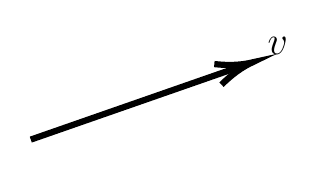
\begin{tikzpicture}[x=0.75pt,y=0.75pt,yscale=-1,xscale=1]
%uncomment if require: \path (0,255); %set diagram left start at 0, and has height of 255

%Straight Lines [id:da7094813320033265] 
\draw [color={rgb, 255:red, 0; green, 0; blue, 0 }  ,draw opacity=1 ][line width=2.25]    (50.01,173.8) -- (152.9,137.94) ;
\draw [shift={(156.68,136.62)}, rotate = 160.79] [color={rgb, 255:red, 0; green, 0; blue, 0 }  ,draw opacity=1 ][line width=2.25]    (17.49,-5.26) .. controls (11.12,-2.23) and (5.29,-0.48) .. (0,0) .. controls (5.29,0.48) and (11.12,2.23) .. (17.49,5.26)   ;

% Text Node
\draw (168.96,128.45) node  [font=\Large,color={rgb, 255:red, 0; green, 0; blue, 0 }  ,opacity=1 ] [align=left] {$\displaystyle \boldsymbol{v}$};


\end{tikzpicture}







\tikzset{every picture/.style={line width=0.75pt}} %set default line width to 0.75pt        

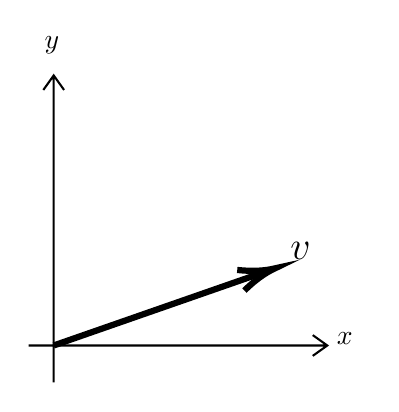
\begin{tikzpicture}[x=0.75pt,y=0.75pt,yscale=-1,xscale=1]
%uncomment if require: \path (0,255); %set diagram left start at 0, and has height of 255

%Shape: Axis 2D [id:dp6210778678969601] 
\draw [color={rgb, 255:red, 0; green, 0; blue, 0 }  ,draw opacity=1 ][line width=0.75]  (37.97,173.8) -- (181.82,173.8)(50.01,43.69) -- (50.01,191.57) (174.82,168.8) -- (181.82,173.8) -- (174.82,178.8) (45.01,50.69) -- (50.01,43.69) -- (55.01,50.69)  ;
%Straight Lines [id:da8210279907873171] 
\draw [color={rgb, 255:red, 0; green, 0; blue, 0 }  ,draw opacity=1 ][line width=2.25]    (50.01,173.8) -- (152.9,137.94) ;
\draw [shift={(156.68,136.62)}, rotate = 160.79] [color={rgb, 255:red, 0; green, 0; blue, 0 }  ,draw opacity=1 ][line width=2.25]    (17.49,-5.26) .. controls (11.12,-2.23) and (5.29,-0.48) .. (0,0) .. controls (5.29,0.48) and (11.12,2.23) .. (17.49,5.26)   ;

% Text Node
\draw (51.34,29.29) node  [font=\normalsize] [align=left] {$\displaystyle y \ $};
% Text Node
\draw (192.5,170.46) node  [font=\normalsize] [align=left] {$\displaystyle x\ $};
% Text Node
\draw (168.96,128.45) node  [font=\Large,color={rgb, 255:red, 0; green, 0; blue, 0 }  ,opacity=1 ] [align=left] {$\displaystyle \boldsymbol{v}$};


\end{tikzpicture}







\tikzset{every picture/.style={line width=0.75pt}} %set default line width to 0.75pt        

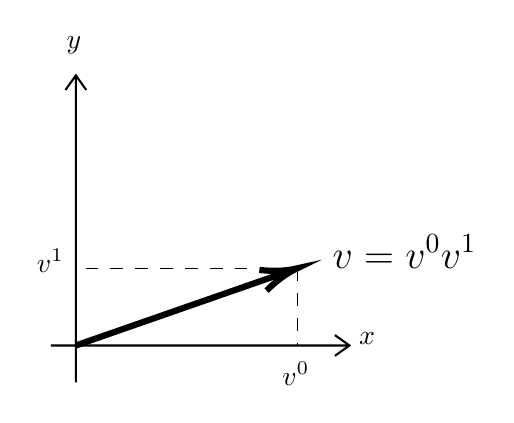
\begin{tikzpicture}[x=0.75pt,y=0.75pt,yscale=-1,xscale=1]
%uncomment if require: \path (0,255); %set diagram left start at 0, and has height of 255

%Shape: Axis 2D [id:dp5057492214774844] 
\draw [color={rgb, 255:red, 0; green, 0; blue, 0 }  ,draw opacity=1 ][line width=0.75]  (37.97,173.8) -- (181.82,173.8)(50.01,43.69) -- (50.01,191.57) (174.82,168.8) -- (181.82,173.8) -- (174.82,178.8) (45.01,50.69) -- (50.01,43.69) -- (55.01,50.69)  ;
%Straight Lines [id:da7094813320033265] 
\draw [color={rgb, 255:red, 0; green, 0; blue, 0 }  ,draw opacity=1 ][line width=2.25]    (50.01,173.8) -- (152.9,137.94) ;
\draw [shift={(156.68,136.62)}, rotate = 160.79] [color={rgb, 255:red, 0; green, 0; blue, 0 }  ,draw opacity=1 ][line width=2.25]    (17.49,-5.26) .. controls (11.12,-2.23) and (5.29,-0.48) .. (0,0) .. controls (5.29,0.48) and (11.12,2.23) .. (17.49,5.26)   ;
%Straight Lines [id:da6786315418220156] 
\draw  [dash pattern={on 4.5pt off 4.5pt}]  (156.68,136.62) -- (156.68,173.33) ;
%Straight Lines [id:da46285115103673846] 
\draw  [dash pattern={on 4.5pt off 4.5pt}]  (156.68,136.62) -- (50.56,136.62) ;

% Text Node
\draw (51.34,29.29) node  [font=\normalsize] [align=left] {$\displaystyle y \ $};
% Text Node
\draw (192.5,170.46) node  [font=\normalsize] [align=left] {$\displaystyle x\ $};
% Text Node
\draw (168.96,128.45) node  [anchor=west, font=\Large,color={rgb, 255:red, 0; green, 0; blue, 0 }  ,opacity=1 ] [align=left] {$\displaystyle \boldsymbol{v}= \pvec{v^0}{v^1}$};
% Text Node
\draw (156.04,187.3) node   [align=left] {$\displaystyle v^{0}$};
% Text Node
\draw (37.71,132.96) node   [align=left] {$\displaystyle v^{1}$};


\end{tikzpicture}






\tikzset{every picture/.style={line width=0.75pt}} %set default line width to 0.75pt        

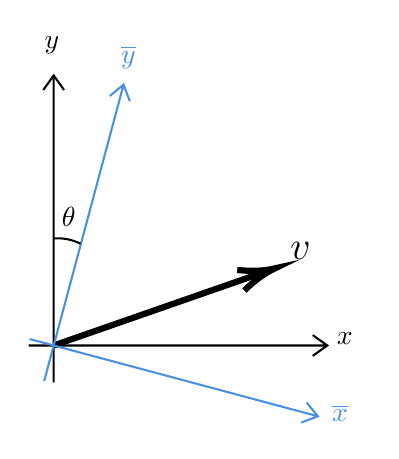
\begin{tikzpicture}[x=0.75pt,y=0.75pt,yscale=-1,xscale=1]
%uncomment if require: \path (0,255); %set diagram left start at 0, and has height of 255

%Shape: Axis 2D [id:dp5382369256645271] 
\draw [color={rgb, 255:red, 0; green, 0; blue, 0 }  ,draw opacity=1 ][line width=0.75]  (37.97,173.8) -- (181.82,173.8)(50.01,43.69) -- (50.01,191.57) (174.82,168.8) -- (181.82,173.8) -- (174.82,178.8) (45.01,50.69) -- (50.01,43.69) -- (55.01,50.69)  ;
%Straight Lines [id:da6942027493640514] 
\draw [color={rgb, 255:red, 0; green, 0; blue, 0 }  ,draw opacity=1 ][line width=2.25]    (50.01,173.8) -- (152.9,137.94) ;
\draw [shift={(156.68,136.62)}, rotate = 160.79] [color={rgb, 255:red, 0; green, 0; blue, 0 }  ,draw opacity=1 ][line width=2.25]    (17.49,-5.26) .. controls (11.12,-2.23) and (5.29,-0.48) .. (0,0) .. controls (5.29,0.48) and (11.12,2.23) .. (17.49,5.26)   ;
%Shape: Axis 2D [id:dp7436814932722576] 
\draw [color={rgb, 255:red, 74; green, 144; blue, 226 }  ,draw opacity=1 ][line width=0.75]  (38.38,170.68) -- (177.33,207.91)(83.68,48.12) -- (45.41,190.97) (171.86,201.27) -- (177.33,207.91) -- (169.27,210.93) (77.04,53.59) -- (83.68,48.12) -- (86.7,56.18)  ;
%Shape: Arc [id:dp22139384946046803] 
\draw  [draw opacity=0][line width=0.75]  (49.71,122.28) .. controls (54.12,121.82) and (58.71,122.67) .. (62.89,124.76) -- (53.96,145.84) -- cycle ; \draw  [color={rgb, 255:red, 0; green, 0; blue, 0 }  ,draw opacity=1 ][line width=0.75]  (49.71,122.28) .. controls (54.12,121.82) and (58.71,122.67) .. (62.89,124.76) ;

% Text Node
\draw (51.34,29.29) node  [font=\normalsize] [align=left] {$\displaystyle y \ $};
% Text Node
\draw (192.5,170.46) node  [font=\normalsize] [align=left] {$\displaystyle x\ $};
% Text Node
\draw (190.24,206.41) node  [font=\normalsize,color={rgb, 255:red, 74; green, 144; blue, 226 }  ,opacity=1 ] [align=left] {$\displaystyle \overline{x} \ $};
% Text Node
\draw (88.2,35.11) node  [font=\normalsize,color={rgb, 255:red, 74; green, 144; blue, 226 }  ,opacity=1 ] [align=left] {$\displaystyle \overline{y} \ $};
% Text Node
\draw (168.96,128.45) node  [font=\Large,color={rgb, 255:red, 0; green, 0; blue, 0 }  ,opacity=1 ] [align=left] {$\displaystyle \boldsymbol{v}$};
% Text Node
\draw (57.21,112) node   [align=left] {$\displaystyle \theta $};


\end{tikzpicture}




\tikzset{every picture/.style={line width=0.75pt}} %set default line width to 0.75pt        

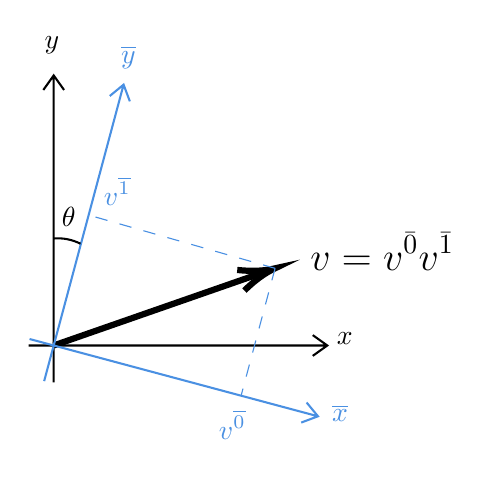
\begin{tikzpicture}[x=0.75pt,y=0.75pt,yscale=-1,xscale=1]
%uncomment if require: \path (0,255); %set diagram left start at 0, and has height of 255

%Shape: Axis 2D [id:dp6852236387651447] 
\draw [color={rgb, 255:red, 0; green, 0; blue, 0 }  ,draw opacity=1 ][line width=0.75]  (37.97,173.8) -- (181.82,173.8)(50.01,43.69) -- (50.01,191.57) (174.82,168.8) -- (181.82,173.8) -- (174.82,178.8) (45.01,50.69) -- (50.01,43.69) -- (55.01,50.69)  ;
%Straight Lines [id:da6926589033039695] 
\draw [color={rgb, 255:red, 0; green, 0; blue, 0 }  ,draw opacity=1 ][line width=2.25]    (50.01,173.8) -- (152.9,137.94) ;
\draw [shift={(156.68,136.62)}, rotate = 160.79] [color={rgb, 255:red, 0; green, 0; blue, 0 }  ,draw opacity=1 ][line width=2.25]    (17.49,-5.26) .. controls (11.12,-2.23) and (5.29,-0.48) .. (0,0) .. controls (5.29,0.48) and (11.12,2.23) .. (17.49,5.26)   ;
%Shape: Axis 2D [id:dp41398149345052926] 
\draw [color={rgb, 255:red, 74; green, 144; blue, 226 }  ,draw opacity=1 ][line width=0.75]  (38.38,170.68) -- (177.33,207.91)(83.68,48.12) -- (45.41,190.97) (171.86,201.27) -- (177.33,207.91) -- (169.27,210.93) (77.04,53.59) -- (83.68,48.12) -- (86.7,56.18)  ;
%Shape: Arc [id:dp42591735237544803] 
\draw  [draw opacity=0][line width=0.75]  (49.71,122.28) .. controls (54.12,121.82) and (58.71,122.67) .. (62.89,124.76) -- (53.96,145.84) -- cycle ; \draw  [color={rgb, 255:red, 0; green, 0; blue, 0 }  ,draw opacity=1 ][line width=0.75]  (49.71,122.28) .. controls (54.12,121.82) and (58.71,122.67) .. (62.89,124.76) ;
%Straight Lines [id:da07735549713184964] 
\draw [color={rgb, 255:red, 74; green, 144; blue, 226 }  ,draw opacity=1 ] [dash pattern={on 4.5pt off 4.5pt}]  (156.68,136.62) -- (140.4,197.6) ;
%Straight Lines [id:da7297712712643412] 
\draw [color={rgb, 255:red, 74; green, 144; blue, 226 }  ,draw opacity=1 ] [dash pattern={on 4.5pt off 4.5pt}]  (156.68,136.62) -- (67.33,111.11) ;

% Text Node
\draw (51.34,29.29) node  [font=\normalsize] [align=left] {$\displaystyle y \ $};
% Text Node
\draw (192.5,170.46) node  [font=\normalsize] [align=left] {$\displaystyle x\ $};
% Text Node
\draw (190.24,206.41) node  [font=\normalsize,color={rgb, 255:red, 74; green, 144; blue, 226 }  ,opacity=1 ] [align=left] {$\displaystyle \overline{x} \ $};
% Text Node
\draw (88.2,35.11) node  [font=\normalsize,color={rgb, 255:red, 74; green, 144; blue, 226 }  ,opacity=1 ] [align=left] {$\displaystyle \overline{y} \ $};
% Text Node
\draw (168.96,128.45) node  [anchor=west, font=\Large,color={rgb, 255:red, 0; green, 0; blue, 0 }  ,opacity=1 ] [align=left] {$\displaystyle \boldsymbol{v} = \pvec{v^{\bar{0}}}{v^{\bar{1}}}$};
% Text Node
\draw (57.21,112) node   [align=left] {$\displaystyle \theta $};
% Text Node
\draw (136.07,212) node  [font=\normalsize,color={rgb, 255:red, 74; green, 144; blue, 226 }  ,opacity=1 ] [align=left] {$\displaystyle v^{\overline{0}}$};
% Text Node
\draw (80.63,99.44) node  [font=\normalsize,color={rgb, 255:red, 74; green, 144; blue, 226 }  ,opacity=1 ] [align=left] {$\displaystyle v^{\overline{1}}$};


\end{tikzpicture}





\begin{figure}[H]
    \centering
    \begin{minipage}[b]{0.49\columnwidth}
        \centering
        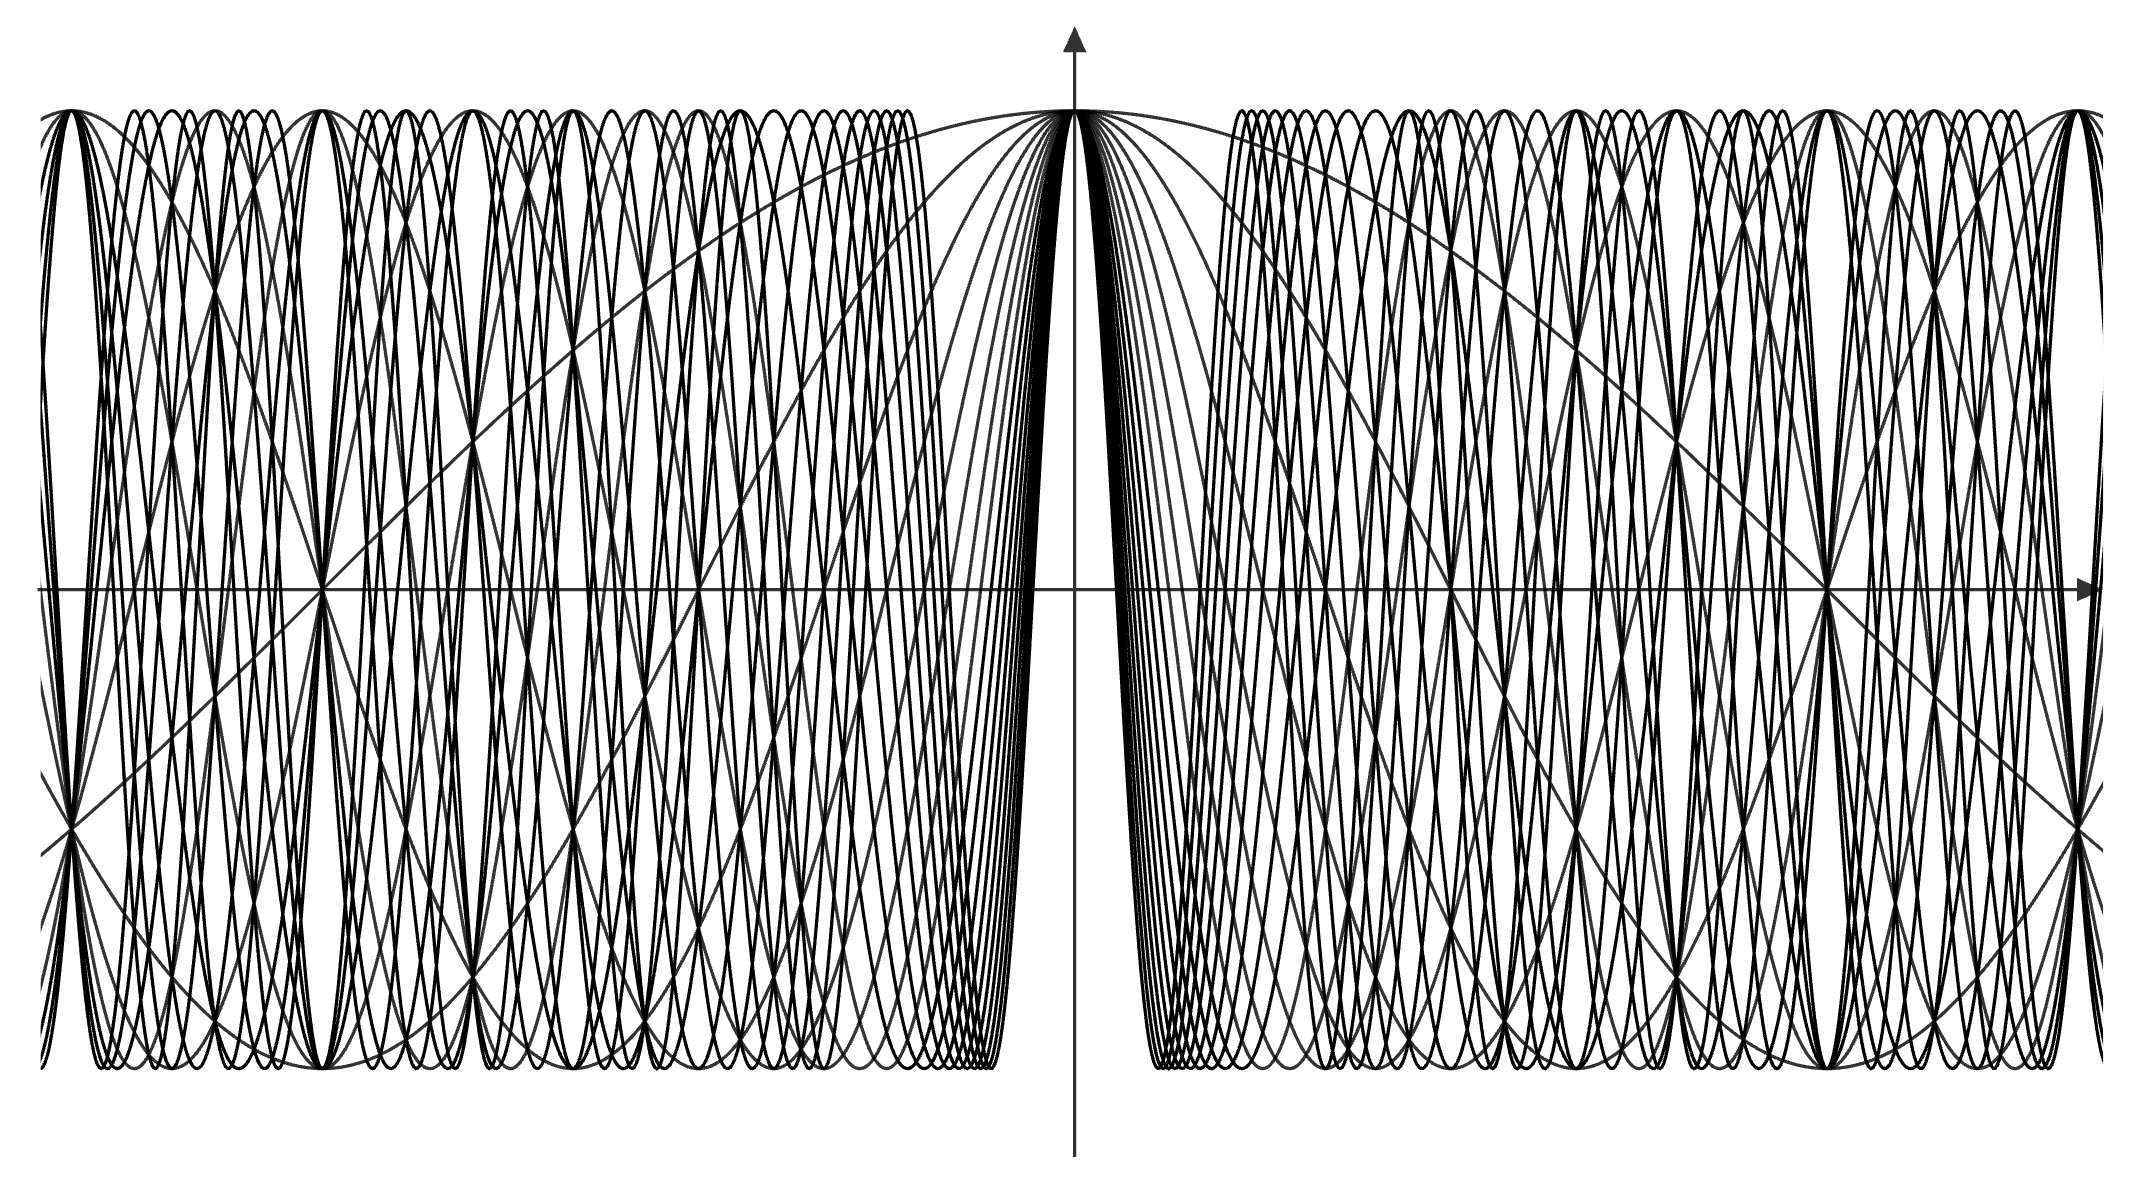
\includegraphics[width=0.8\columnwidth]{./images/waves.png}
        \caption{\(\cos{nx}\)}
        \label{fig:a}
    \end{minipage}
    \begin{minipage}[b]{0.49\columnwidth}
        \centering
        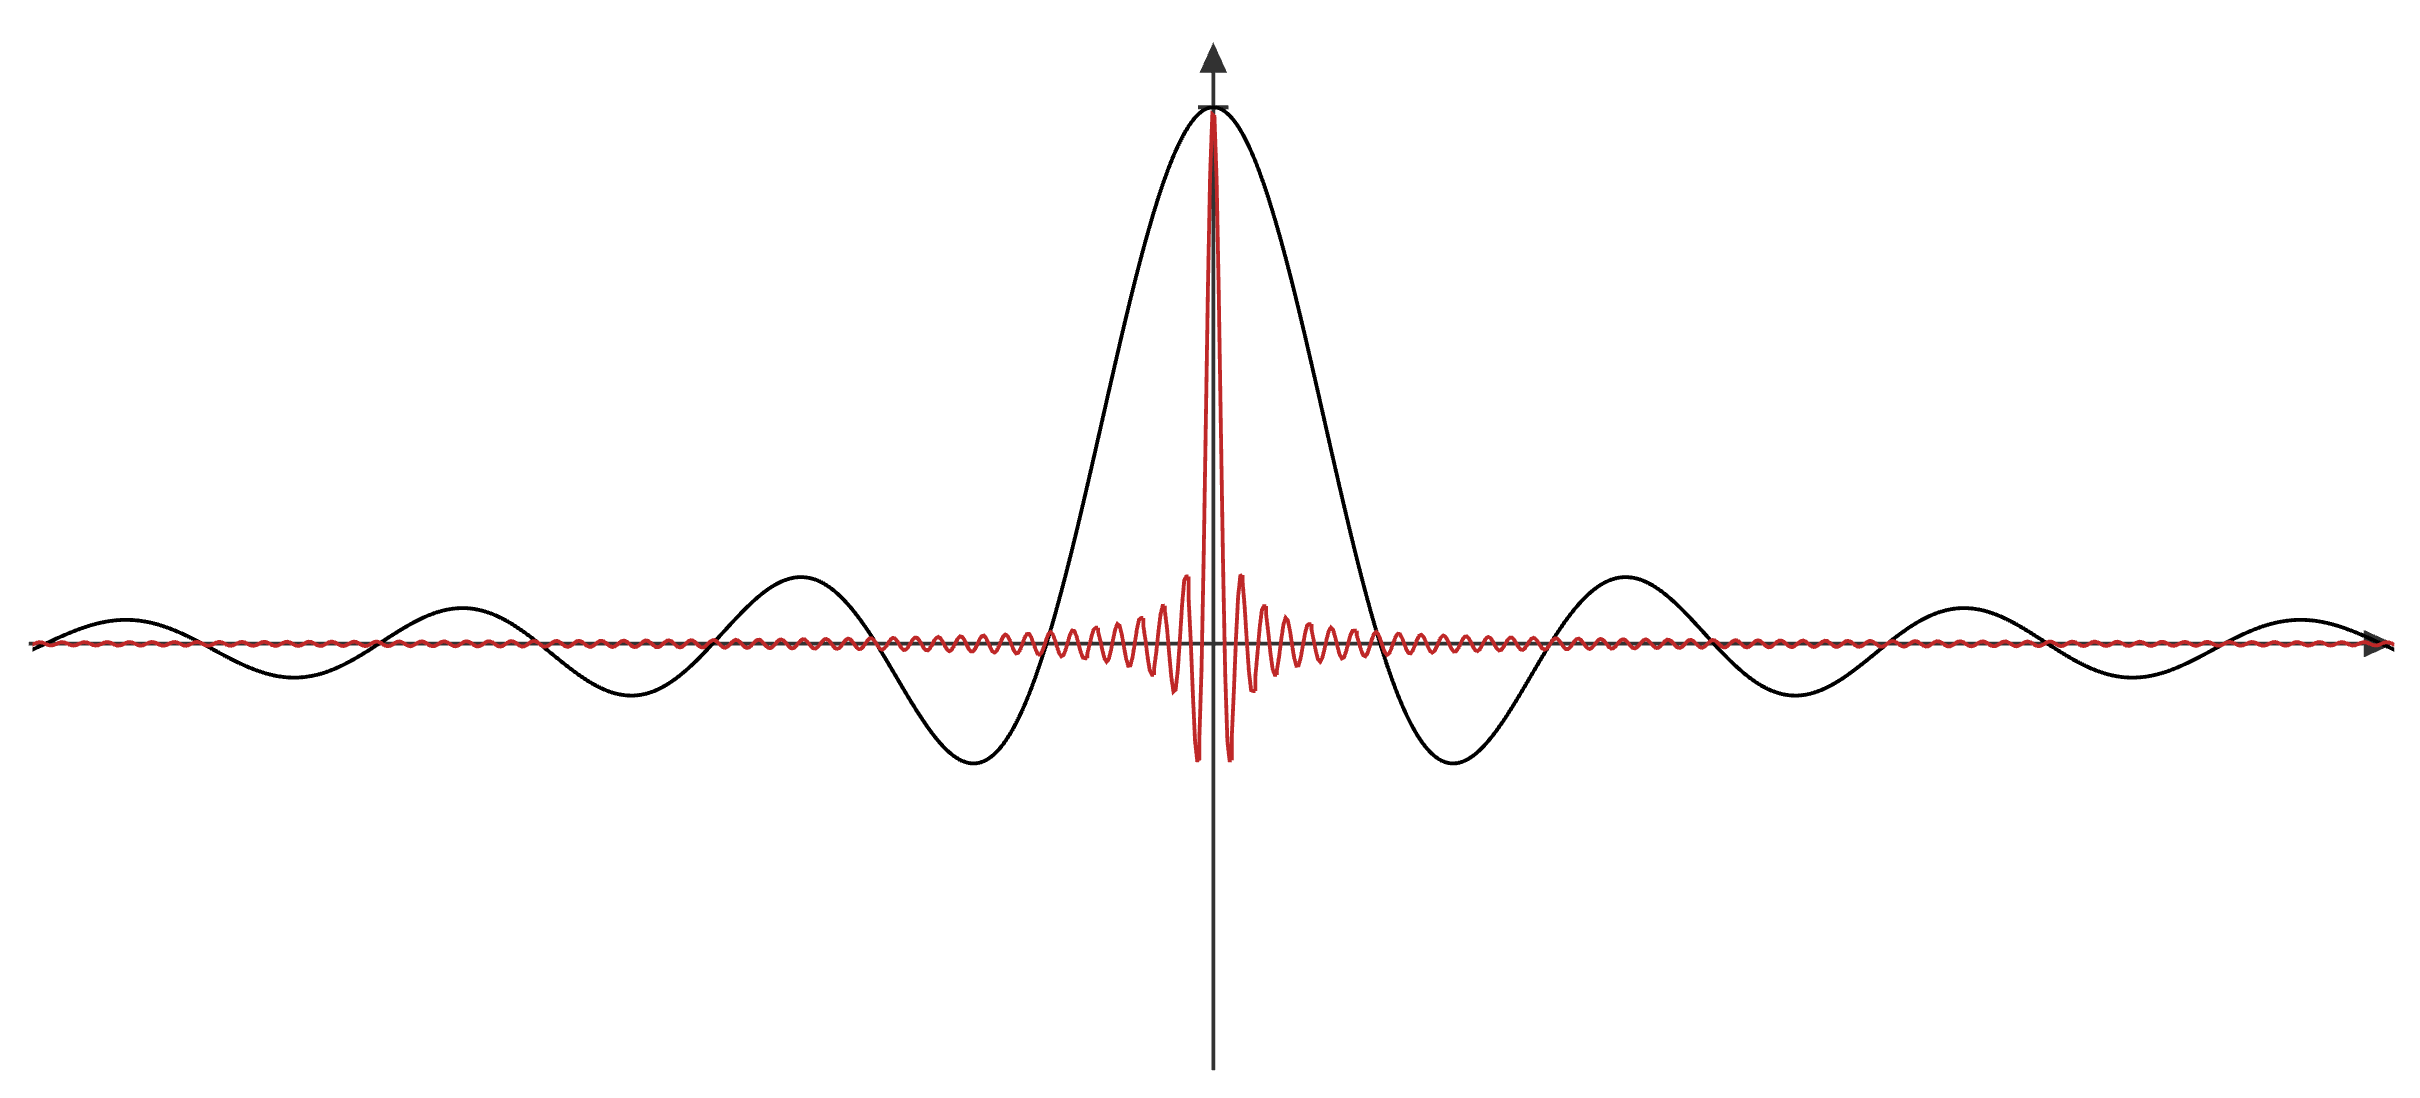
\includegraphics[width=0.95\columnwidth]{./images/added_waves.png}
        \caption{\(\cos{nx}\)のたし合わせ}
        \label{fig:b}
    \end{minipage}
\end{figure}





\begin{tikzpicture}[
    >=latex, % 矢印のスタイル
    ]

    % --- 座標軸 ---
    % x軸
    \draw[->] (-2.5,0) -- (2.5,0) node[below left] {$x$};
    % y軸
    \draw[->] (0,-0.5) -- (0,3.5) node[below left] {$y$};

    % 原点のラベル
    \node[below left] at (0,0) {$0$};

    % --- デルタ関数 ---
    % x=0 の位置に上向きの矢印を描画
    % thick で線を太くし、矢印の長さ (ここでは 0 から 3 まで) を調整
    \draw[very thick, color={rgb, 255:red, 200; green, 0; blue, 30}] (0,0) -- (0,3) node[anchor=south west] {$\delta(x)$};
    \draw[very thick, color={rgb, 255: red, 200; green, 0; blue, 30}] (-2,0) -- (2,0);

    % --- (オプション)軸の目盛り ---
    % \foreach \x in {-2,-1,1,2}
    %     \draw (\x,0.1) -- (\x,-0.1) node[below] {$\x$};
    % \foreach \y in {1,2,3}
    %     \draw (0.1,\y) -- (-0.1,\y) node[left] {$\y$};

\end{tikzpicture}





\tikzset{every picture/.style={line width=0.75pt}} %set default line width to 0.75pt        

\begin{tikzpicture}[x=0.75pt,y=0.75pt,yscale=-1,xscale=1]
%uncomment if require: \path (0,255); %set diagram left start at 0, and has height of 255

%Shape: Axis 2D [id:dp11470844755900778] 
\draw [color={rgb, 255:red, 0; green, 0; blue, 0 }  ,draw opacity=1 ][line width=0.75]  (37.97,173.8) -- (181.82,173.8)(50.01,43.69) -- (50.01,191.57) (174.82,168.8) -- (181.82,173.8) -- (174.82,178.8) (45.01,50.69) -- (50.01,43.69) -- (55.01,50.69)  ;
%Straight Lines [id:da09191499177354956] 
\draw [color={rgb, 255:red, 0; green, 0; blue, 0 }  ,draw opacity=1 ][line width=2.25]    (50.01,173.8) -- (152.9,137.94) ;
\draw [shift={(156.68,136.62)}, rotate = 160.79] [color={rgb, 255:red, 0; green, 0; blue, 0 }  ,draw opacity=1 ][line width=2.25]    (17.49,-5.26) .. controls (11.12,-2.23) and (5.29,-0.48) .. (0,0) .. controls (5.29,0.48) and (11.12,2.23) .. (17.49,5.26)   ;

% Text Node
\draw (51.34,29.29) node  [font=\normalsize] [align=left] {$\displaystyle y \ $};
% Text Node
\draw (192.5,170.46) node  [font=\normalsize] [align=left] {$\displaystyle x\ $};
% Text Node
\draw (164.36,106.33) node [anchor=north west][inner sep=0.75pt]  [font=\Large,color={rgb, 255:red, 0; green, 0; blue, 0 }  ,opacity=1 ] [align=left] {退勤};


\end{tikzpicture}






\tikzset{every picture/.style={line width=0.75pt}} %set default line width to 0.75pt        

\begin{tikzpicture}[x=0.75pt,y=0.75pt,yscale=-1,xscale=1]
%uncomment if require: \path (0,261); %set diagram left start at 0, and has height of 261

%Shape: Axis 2D [id:dp442515431015299] 
\draw [color={rgb, 255:red, 0; green, 0; blue, 0 }  ,draw opacity=1 ][line width=0.75]  (37.97,173.8) -- (181.82,173.8)(50.01,43.69) -- (50.01,191.57) (174.82,168.8) -- (181.82,173.8) -- (174.82,178.8) (45.01,50.69) -- (50.01,43.69) -- (55.01,50.69)  ;
%Straight Lines [id:da8185322428169859] 
\draw [color={rgb, 255:red, 0; green, 0; blue, 0 }  ,draw opacity=1 ][line width=2.25]    (50.01,173.8) -- (152.9,137.94) ;
\draw [shift={(156.68,136.62)}, rotate = 160.79] [color={rgb, 255:red, 0; green, 0; blue, 0 }  ,draw opacity=1 ][line width=2.25]    (17.49,-5.26) .. controls (11.12,-2.23) and (5.29,-0.48) .. (0,0) .. controls (5.29,0.48) and (11.12,2.23) .. (17.49,5.26)   ;
%Straight Lines [id:da9683046472088979] 
\draw  [dash pattern={on 4.5pt off 4.5pt}]  (156.68,136.62) -- (156.68,173.33) ;
%Straight Lines [id:da6009378515005339] 
\draw  [dash pattern={on 4.5pt off 4.5pt}]  (156.68,136.62) -- (50.56,136.62) ;

% Text Node
\draw (51.34,29.29) node  [font=\normalsize] [align=left] {$\displaystyle y \ $};
% Text Node
\draw (192.5,170.46) node  [font=\normalsize] [align=left] {$\displaystyle x\ $};
% Text Node
\draw (164.36,106.33) node [anchor=north west][inner sep=0.75pt]  [font=\Large,color={rgb, 255:red, 0; green, 0; blue, 0 }  ,opacity=1 ] [align=left] {退勤};
% Text Node
\draw (136,177.33) node [anchor=north west][inner sep=0.75pt]   [align=left] {9000};
% Text Node
\draw (8,125.67) node [anchor=north west][inner sep=0.75pt]   [align=left] {52e4};


\end{tikzpicture}







\tikzset{every picture/.style={line width=0.75pt}} %set default line width to 0.75pt        

\begin{tikzpicture}[x=0.75pt,y=0.75pt,yscale=-1,xscale=1]
%uncomment if require: \path (0,255); %set diagram left start at 0, and has height of 255

%Shape: Axis 2D [id:dp729365571863981] 
\draw [color={rgb, 255:red, 0; green, 0; blue, 0 }  ,draw opacity=1 ][line width=0.75]  (37.97,173.8) -- (181.82,173.8)(50.01,43.69) -- (50.01,191.57) (174.82,168.8) -- (181.82,173.8) -- (174.82,178.8) (45.01,50.69) -- (50.01,43.69) -- (55.01,50.69)  ;
%Straight Lines [id:da7301841569805996] 
\draw [color={rgb, 255:red, 0; green, 0; blue, 0 }  ,draw opacity=1 ][line width=2.25]    (50.01,173.8) -- (152.9,137.94) ;
\draw [shift={(156.68,136.62)}, rotate = 160.79] [color={rgb, 255:red, 0; green, 0; blue, 0 }  ,draw opacity=1 ][line width=2.25]    (17.49,-5.26) .. controls (11.12,-2.23) and (5.29,-0.48) .. (0,0) .. controls (5.29,0.48) and (11.12,2.23) .. (17.49,5.26)   ;
%Straight Lines [id:da42045955917608224] 
\draw  [dash pattern={on 4.5pt off 4.5pt}]  (156.68,136.62) -- (156.68,173.33) ;
%Straight Lines [id:da52711562427977] 
\draw  [dash pattern={on 4.5pt off 4.5pt}]  (156.68,136.62) -- (50.56,136.62) ;
%Shape: Axis 2D [id:dp5456016543299301] 
\draw [color={rgb, 255:red, 74; green, 144; blue, 226 }  ,draw opacity=1 ][line width=0.75]  (38.33,170.71) -- (177.27,207.94)(83.63,48.15) -- (45.35,191) (171.8,201.3) -- (177.27,207.94) -- (169.21,210.96) (76.99,53.62) -- (83.63,48.15) -- (86.65,56.21)  ;
%Straight Lines [id:da8637663417126374] 
\draw [color={rgb, 255:red, 74; green, 144; blue, 226 }  ,draw opacity=1 ] [dash pattern={on 4.5pt off 4.5pt}]  (156.63,136.65) -- (140.34,197.63) ;
%Straight Lines [id:da6003255838629276] 
\draw [color={rgb, 255:red, 74; green, 144; blue, 226 }  ,draw opacity=1 ] [dash pattern={on 4.5pt off 4.5pt}]  (156.63,136.65) -- (67.28,111.14) ;

% Text Node
\draw (51.34,29.29) node  [font=\normalsize] [align=left] {$\displaystyle y \ $};
% Text Node
\draw (192.5,170.46) node  [font=\normalsize] [align=left] {$\displaystyle x\ $};
% Text Node
\draw (164.36,106.33) node [anchor=north west][inner sep=0.75pt]  [font=\Large,color={rgb, 255:red, 0; green, 0; blue, 0 }  ,opacity=1 ] [align=left] {退勤};
% Text Node
\draw (116.8,198.07) node [anchor=north west][inner sep=0.75pt]  [color={rgb, 255:red, 74; green, 144; blue, 226 }  ,opacity=1 ] [align=left] {91de};
% Text Node
\draw (190.18,206.44) node  [font=\normalsize,color={rgb, 255:red, 74; green, 144; blue, 226 }  ,opacity=1 ] [align=left] {$\displaystyle \overline{x} \ $};
% Text Node
\draw (88.14,35.14) node  [font=\normalsize,color={rgb, 255:red, 74; green, 144; blue, 226 }  ,opacity=1 ] [align=left] {$\displaystyle \overline{y} \ $};
% Text Node
\draw (72.4,89) node [anchor=north west][inner sep=0.75pt]  [color={rgb, 255:red, 74; green, 144; blue, 226 }  ,opacity=1 ] [align=left] {8bce};


\end{tikzpicture}






\tikzset{every picture/.style={line width=0.75pt}} %set default line width to 0.75pt        

\begin{tikzpicture}[x=0.75pt,y=0.75pt,yscale=-1,xscale=1]
%uncomment if require: \path (0,255); %set diagram left start at 0, and has height of 255

%Shape: Axis 2D [id:dp9112509217470328] 
\draw [color={rgb, 255:red, 0; green, 0; blue, 0 }  ,draw opacity=1 ][line width=0.75]  (37.97,173.8) -- (181.82,173.8)(50.01,43.69) -- (50.01,191.57) (174.82,168.8) -- (181.82,173.8) -- (174.82,178.8) (45.01,50.69) -- (50.01,43.69) -- (55.01,50.69)  ;
%Straight Lines [id:da773425450806867] 
\draw [color={rgb, 255:red, 74; green, 144; blue, 226 }  ,draw opacity=1 ][line width=2.25]    (50.01,173.8) -- (152.9,137.94) ;
\draw [shift={(156.68,136.62)}, rotate = 160.79] [color={rgb, 255:red, 74; green, 144; blue, 226 }  ,draw opacity=1 ][line width=2.25]    (17.49,-5.26) .. controls (11.12,-2.23) and (5.29,-0.48) .. (0,0) .. controls (5.29,0.48) and (11.12,2.23) .. (17.49,5.26)   ;
%Shape: Axis 2D [id:dp4449016124553483] 
\draw [color={rgb, 255:red, 74; green, 144; blue, 226 }  ,draw opacity=1 ][line width=0.75]  (38.33,170.71) -- (177.27,207.94)(83.63,48.15) -- (45.35,191) (171.8,201.3) -- (177.27,207.94) -- (169.21,210.96) (76.99,53.62) -- (83.63,48.15) -- (86.65,56.21)  ;
%Straight Lines [id:da5752027494469741] 
\draw [color={rgb, 255:red, 0; green, 0; blue, 0 }  ,draw opacity=1 ][line width=2.25]    (50.01,173.8) -- (142.79,105.05) ;
\draw [shift={(146,102.67)}, rotate = 143.46] [color={rgb, 255:red, 0; green, 0; blue, 0 }  ,draw opacity=1 ][line width=2.25]    (17.49,-5.26) .. controls (11.12,-2.23) and (5.29,-0.48) .. (0,0) .. controls (5.29,0.48) and (11.12,2.23) .. (17.49,5.26)   ;

% Text Node
\draw (51.34,29.29) node  [font=\normalsize] [align=left] {$\displaystyle y \ $};
% Text Node
\draw (192.5,170.46) node  [font=\normalsize] [align=left] {$\displaystyle x\ $};
% Text Node
\draw (190.18,206.44) node  [font=\normalsize,color={rgb, 255:red, 74; green, 144; blue, 226 }  ,opacity=1 ] [align=left] {$\displaystyle \overline{x} \ $};
% Text Node
\draw (88.14,35.14) node  [font=\normalsize,color={rgb, 255:red, 74; green, 144; blue, 226 }  ,opacity=1 ] [align=left] {$\displaystyle \overline{y} \ $};
% Text Node
\draw (160.8,112.33) node [anchor=north west][inner sep=0.75pt]  [color={rgb, 255:red, 74; green, 144; blue, 226 }  ,opacity=1 ] [align=left] {$\displaystyle \ \begin{pmatrix}
91\mathrm{de}\\
\mathrm{8bce}
\end{pmatrix}$ };
% Text Node
\draw (237,66) node [anchor=north west][inner sep=0.75pt]   [align=left] {釞诎};
% Text Node
\draw (160.8,54.33) node [anchor=north west][inner sep=0.75pt]  [color={rgb, 255:red, 0; green, 0; blue, 0 }  ,opacity=1 ] [align=left] {$\displaystyle \ \begin{pmatrix}
91\mathrm{de}\\
\mathrm{8bce}
\end{pmatrix}$ };
% Text Node
\draw (237,124) node [anchor=north west][inner sep=0.75pt]   [align=left] {\textcolor[rgb]{0.29,0.56,0.89}{退勤}};


\end{tikzpicture}



\end{document}